\section{Introduction and Goals}

According to the \acrfull{fao} in 2019 931 millions tonnes of food were wasted \cite{refart:FAOFW}. This has
environmental, but special social consequences. In a world were approximately 9.9\% of the \cite{refart:AAHWH}
population suffers from hunger that waste percentage sounds paradoxal.

According to \acrfull{un} 5\% of the globally food loss and waste comes from restaurants \cite{refart:UNSP}. 
The solution for this problem muss be locally applied so its effects can be seen in a global structure. To do so we
propose to develop a mobile application that connects restaurants, bakeries and or pastries to clients. 
The former would offer their remaining products, which are still consumable, prior to the closing time, to a small price 
and the latter would browser in the app to find which shops are offering products. 

 
\subsection{Design Purpose}

The main purpose of this architecture is creating exploratory prototype of an \gls{app}. We aim to test it with potential 
\gls{stakeholder} and regions to analyze the general their acceptance and wishes \cite{refbook:DSHC} and get a fast feedback. 

This prototype will also make it feasible to identify unknown needs an wishes of the potential \gls{stakeholder}, so we can eventually
increase the scope of functionality. Exploring this domain will also provide us with information regarding the behavior 
of our \gls{stakeholder} when it comes to buying and serving food that would be wasted, but is still consumable.

\subsection{Primary Functionality} \label{Primary_Functionality}

From the following use cases we will be able to define the primary functionality of our application and furthermore 
identify its main quality attributes 

% Object: put figure beside the table

\begin{table}[H]
    \begin{tabularx}{\textwidth}{lX}
    \toprule
    Use Case & Description  \\
    \midrule
    UC-1: Register as \gls{client} & The \gls{client} register an e-mail address.\\
    UC-2: Login & The \gls{client} logins in to the system. \\
    UC-3: Place an order & The \gls{client} chooses a \gls{provider}. \\
    UC-4: Register payment & The \gls{client} register a payment method. \\
    UC-5: Register as \gls{provider} & The \gls{provider} register their facility and products. \\
    UC-6: Update availability & The \gls{provider} upload their availability to provide a product. \\
    \bottomrule
    \end{tabularx}
\end{table}

Those use cases are also represented in the following use case diagram:

\begin{figure}[H]
    \centering
    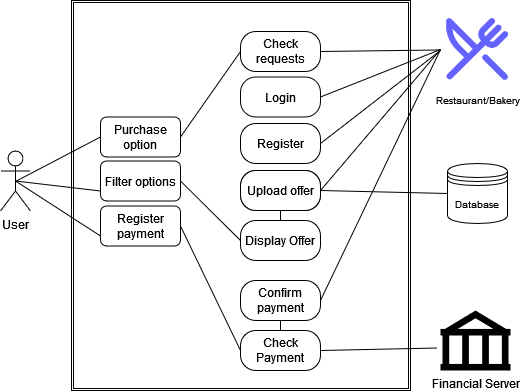
\includegraphics[width=0.9\textwidth]{assets/preliminary_use_case.png}
    \caption{Preliminary functions}
    \label{fig:preliminary_use_case}
\end{figure}


\subsection{Quality Attributes}

With the given use cases we will then be able to define the major quality attributes that are involved in the 
development of this application. We want those qualities to be measurable and testable so we can verify if the 
system meets the needs our \glsplural{stakeholder} \cite{refbook:DSHC}.

\begin{table}[H]
    \setstretch{1.0}
    \begin{tabularx}{\textwidth}{lcXc}
        \toprule
        ID & Quality Attribute & Scenario & Associated Use Case  \\
        \midrule
        QA-1 & Performance & A \gls{client} register their e-mail address and he can immediate browse in the app. & UC-1 \\
        QA-2 & Performance & A \gls{client} opens the app and he can immediate browse in the app. & UC-2 \\
        QA-3 & Performance & A \gls{client} choose a \gls{provider} and place his order. After the confirmation
        of payment, a push-message is displayed in the app confirming the purchase. & UC-3 \\
        QA-4 & \textit{[to be defined]} & A \gls{client}  register his credit card or select another payment method and the
        confirmation as soon as he confirmed with his \gls{provider}. & UC-4 \\
        QA-5 & Usability & A \gls{provider} is able to register his company, specify the kind of products he offers and upload
        a logo or picture of his shop. & UC-5 \\
        QA-6 & Usability & A \gls{provider} is able to update in the app if he is offering for that day any product. &  UC-6 \\
        QA-7 & Interoperability & A \gls{client} can register his e-mail using another account (Google, Microsoft, Facebook)
        in a federated environment & UC01 \\
        QA-8 & Interoperability & A \gls{client} can pay the order using a \gls{mobile payment gateway} (i.e. Stripe, Square, PayPay, 
        SecurePay) & UC-1 \\
        \bottomrule
    \end{tabularx}
\end{table}

\newpage
The defined quality attributes are represented in the following scenarios:

\begin{table}[H]
    \setstretch{1.0}
    \begin{tabularx}{\textwidth}{|c|X|}
        \hline
        \multicolumn{2}{c}{\textbf{Performance}} \\
        \hline
        \toprule
        \multicolumn{1}{c}{Scenario} & \multicolumn{1}{c}{Value} \\
        \midrule
        Source & \gls{client}  \\
        Stimulus & wishes to create an account \\
        Artifact & platform \\
        Environment & runtime \\
        Response & immediate access to the app \\
        Response Measure & time between confirmation and access \\
         & \\
        Source & \gls{client}  \\
        Stimulus & wants to search fo restaurants or bakeries \\
        Artifact & platform \\
        Environment & peak period, between 6 and 7 pm on Friday \\
        Response & immediate access to the offers \\
        Response Measure & how quick does the \gls{client}  get an updated regarding availability of products \\
        & \\
        Source & \gls{client}  \\
        Stimulus & place an order \\
        Artifact & platform \\
        Environment & peak period, between 6 and 7 pm on Friday \\
        Response & confirmation of the purchase after the payment \\
        Response Measure & time between confirmation of the payment and confirmation of the order \\
        \bottomrule
    \end{tabularx}
\end{table}


\begin{table}[H]
    \setstretch{1.0}
    \begin{tabularx}{\textwidth}{|c|X|}
        \hline
        \multicolumn{2}{c}{\textbf{Usability}} \\
        \hline
        \toprule
        \multicolumn{1}{c}{Scenario} & \multicolumn{1}{c}{Value} \\
        \midrule
        Source & \gls{provider} \\
        Stimulus & wants to offer his remaining products in the app \\
        Artifact & platform \\
        Environment & working time, during afternoon \\
        Response & offer available in the app \\
        Response Measure & How long did the registration and upload process took? Were all necessary information
        available in the app or did the \gls{provider} need to search it outside the app? How long did the registration
        process took? \\
         & \\
        Source & Registered \gls{provider} \\
        Stimulus & wants wants to make a last minute offer \\
        Artifact & platform \\
        Environment & peak period, between 6 and 7 pm on Friday \\
        Response & immediate availability of the offer in the app \\
        Response Measure & how long did it take for the \gls{provider} to upload the offer? Was it easy to input all
        necessary information like, quantity, location and take-away time? Can he do it without any burden? \\
        \bottomrule
    \end{tabularx}
\end{table}

\newpage
\subsection{Constraints}

In general, we can say that constrains are burdens to the development of the project. They define a set of non-negotiable
rules that must be exist \cite{refonline:EFAD}. 

In this project we must distinguish between Technical and Business Constraints. The former describes specific elements
of the project, like programming language, released platform (i.e. operational systems) and technical decisions related to 
the functionalities. The latter deals with management elements\cite{refonline:EFAD} such time, budget and team.


\begin{table}[htb]
    \setstretch{1.0}
    \begin{tabularx}{\textwidth}{lclX}
        \toprule
        ID & Constraint & Category & Description \\
        \midrule
        CT-1 & Programming Language & Technical & Java, Kotlin, iOS, Swift \\
        CT-2 & Platform & Technical & Android, IoS \\
        CT-3 & Payment & Technical & Creating own framework or integrating with existing one (Google Pay, Apple Pay, PayPall) \\
        CT-4 & Login & Technical & Using or not federation or creating own login system  \\
        CT-5 & Time to first prototype release & Business & How long until a first prototype that can be tested wir real users  \\
        CT-6 & Testing time & Business & Time window to test general acceptance \\
        CT-7 & Budget & Business & To maintain a team during the testing phase \\
        CT-8 & Team & Business & To analyze the main usage of the app for further development \\
        \bottomrule
    \end{tabularx}
\end{table}







%https://medium.com/@janerikfra/architectural-drivers-in-modern-software-architecture-cb7a42527bf2 (important)
% https://www.ecs.csun.edu/~rlingard/COMP684/Example2SoftArch.htm
% https://upcommons.upc.edu/bitstream/handle/2099.1/18373/90629.pdf

% Registration Process for Clients QA1
% Registration Process for Restaurants/Backery QA2
% Login Clients QA3
% Login Restaurant/Backery QA4
% Upload offers QA6
% Purchase QA6
% Receive Confirmation QA7

% Performance
% After upload offer, how long until displyed QA8

% Usuability
% Registration for Client: using existing account or Name/email
% Registration for Restaurant/bakery: Upload name, picture, location and type of products

% Purchase client: choose available RA-options
% Payment: register card, use existing accounts (paypal/google pay)

% Upload offer RA: registered RAs activate that they are offering
% Receive order: after payment confirmed, RA recieves order


% Availability

% Modifiability
